%% LaTeX Beamer presentation template (requires beamer package)
%% see http://bitbucket.org/rivanvx/beamer/wiki/Home
%% idea contributed by H. Turgut Uyar
%% template based on a template by Till Tantau
%% this template is still evolving - it might differ in future releases!

%%	  \begin{itemize}
%%	    \item
%%	  \end{itemize}

\documentclass{beamer}
\setcounter{tocdepth}{2}
\mode<presentation>
{
\usetheme{Warsaw}

\setbeamercovered{transparent}
}

\usepackage[english]{babel}
\usepackage[latin1]{inputenc}

% font definitions, try \usepackage{ae} instead of the following
% three lines if you don't like this look
%\usepackage{ae}
\usepackage{ae}

\usepackage[T1]{fontenc}
\usepackage{graphicx}                    %   for imported graphics
\usepackage{amsmath}                     %%
\usepackage{amsfonts}                    %%  for AMS mathematics
\usepackage{amssymb}                     %%
\usepackage{amsthm}
\usepackage{hyperref}


\title[Validation of Magnetospheric MHD Models]{Validation of
Magnetospheric Magnetohydrodynamic Models}
\author{Brian Curtis}
\institute[Universities of]
{
School of Physics Astronomy and Computational Sciences\\
George Mason University}
\date{April 23rd, 2014 / Final Defense }
\subject{Dissertation}


\begin{document}

\begin{frame}
\titlepage
\end{frame}

\begin{frame}
\frametitle{Special Recognition}
\begin{figure}
	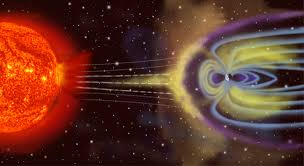
\includegraphics[scale=.5]{images/overview.jpg}
\end{figure}
\textbf{Dissertation Director: Dr. Robert Weigel}\\
\textbf{Dissertation Committee:}
\begin{itemize}
  \item Dr. Jie Zhang
  \item Dr. Art Poland
  \item Dr. Ruixin Yang
\end{itemize}
\end{frame}

\begin{frame}[shrink]
\frametitle{Outline}
\tableofcontents
\end{frame}

\section{Introduction}

\subsection{Motivation}
\begin{frame}[label=Motivation]
\frametitle{Motivation}
\begin{enumerate}
  \item<1> Interest in using MHD models for operational forecasting;
  very little validation is done.
  \begin{itemize}
    \item Most common: in-situ data analysis.
    \item Comprehensive inter-model comparison is not done.
  \end{itemize}
  \item<2> Want understanding of MHD magnetosphere sensitivity to
  initial solar wind conditions.
  \begin{itemize}
    \item Sensitivities not looked into yet.
  \end{itemize}
  \item<3> Want a better understanding of MHD model differences.
  \begin{itemize}
	\item New tool in analyzing two model outputs: Differences.
  \end{itemize}
\end{enumerate}
\end{frame}

% Difficult to model the magnetosphere over an 11 year cycle today, GEM
% challenge is only 6-8 events, each event is unique, documenting the tendencies
% of models gives a reference to model developers as to why a model does poorly
\begin{frame}[label=Summary]
\frametitle{Summary}
\begin{enumerate}
  \item This new inter-model difference comparison, with future work will offer
  a new perspective to model developers in understanding reasoning behind
  results from in-situ data analysis.
  \item MHD models are very sensitive in response to initial conditions. Found
  regions of inconsistencies in these numerical models. For example high
  compression gave three very different results.
  \item Differences between models are large. The ring current has an effect on
  the BATS-R-US output and more validation is still needed to determine the causes
  of these differences. For example, changes in preconditioning times.
\end{enumerate}

\end{frame}


\subsection{Experiments}
\begin{frame}[label=Experiments]
\frametitle{Experiments}
\begin{enumerate}
  \item Response to a change in solar wind $B_z$ from positive to negative.
  (Addresses all motivations)
  \item The influence of preconditioning on MHD magnetospheric models.
  (Addresses motivations 1 and 3)
  \item How magnetospheric MHD models differ in their response to
  extreme solar wind conditions. (Addresses all motivations)
\end{enumerate}
\end{frame}


\subsection{Space Weather}
\begin{frame}
\frametitle{Space Weather}
\centering 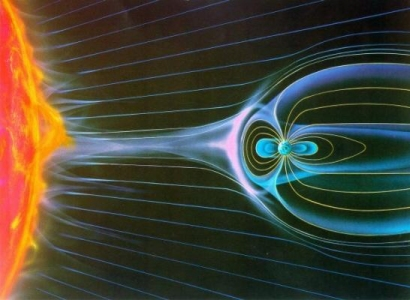
\includegraphics[scale=0.3]{images/NASA_BigPicture.jpg}

\textbf{Space weather:} The term used to describe the current state of the
space environment involving the influence of particles traveling outward from the Sun
on objects in the heliosphere, magnetosphere, ionosphere and thermosphere
(Thompson, 2000)

\end{frame}
\section{Magnetospheric Magnetohydrodynamics}
\subsection{Earth's Magnetosphere}

\begin{frame}
\frametitle{Earth's Magnetosphere}
\begin{figure}
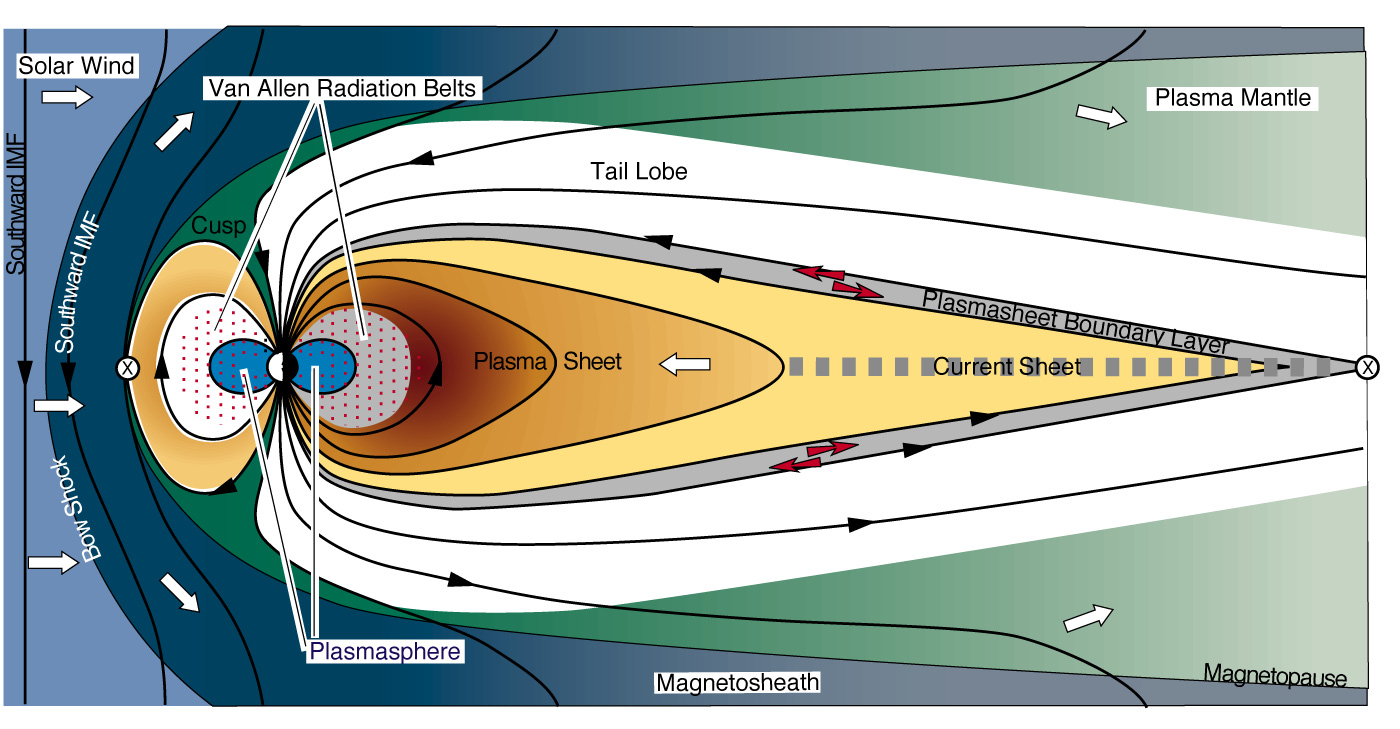
\includegraphics[scale=0.21]{images/Rice_Magnetosphere.jpg}
\end{figure}

\begin{itemize}
  \item Shape determined from a balance between kinetic pressure from the solar
  wind and magnetic pressure from Earth's magnetic field.
  \item IMF direction has most influence on magnetospheric response.
  \item Fluctuates between a bell and teardrop shape.
  \item Reconnection most supported theory for energy transfer in magnetosphere.
\end{itemize}

\end{frame}

\subsection{Magnetohydrodynamics}

\begin{frame}[shrink]
\frametitle{Magnetohydrodynamics}
\begin{tabular}{p{0.5\textwidth}p{0.5\textwidth}}
\begin{itemize}
  \item[] \textbf{Magnetohydrodynamics}
  \item Start with Boltzmann equation for single species.
  \item Invoke conservation of Mass, Momentum, Energy.
  \item Conservation equations summed over all species, treated as a single
  fluid.
  \item Use Maxwell's Equations:
  \begin{itemize}
    \item Gauss' Law.
    \item Gauss' Law for Magnetism.
    \item Faraday's Law.
    \item Ampere's Law.
  \end{itemize}
  
\end{itemize}
 &
\begin{itemize}
  \item[] \textbf{Ideal MHD}
  \item The time derivative of E is small
  \item Isotropic Pressure
  \item Charge neutrality
  \item Neglect small terms
  \item Single ion flow with collision term approximation
  \item Perfect conductivity
\end{itemize}

\begin{itemize}
  \item[] \textbf{Implementation}
  \item Grid Choice
  \item Discretization
\end{itemize}
\end{tabular}
\end{frame}

\subsection{Magnetospheric MHD Models}
\begin{frame}
\frametitle{Modeling}
\centering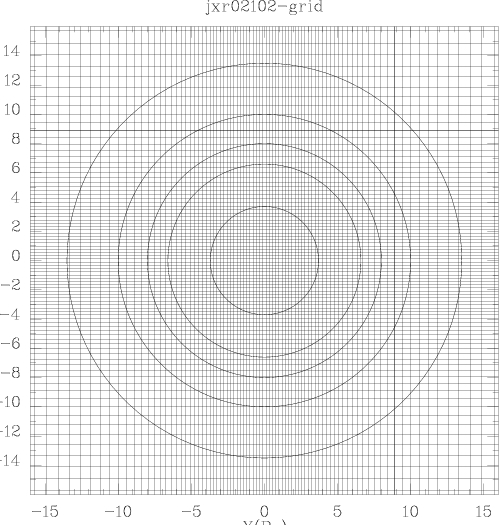
\includegraphics[scale=0.2]{images/StretchedCartesian.jpg}
\begin{itemize}
  \item Grid Choice: Uniform/Stretched Cartesian, SAMR
  \item Boundary/Initial Conditions
  \item Discretization: Finite Differences, Finite Volumes, Finite Elements.
\end{itemize}

\end{frame}

\begin{frame}
\frametitle{Chosen MHD Models}
\begin{tabular}{p{0.4\textwidth}p{0.5\textwidth}}
\centering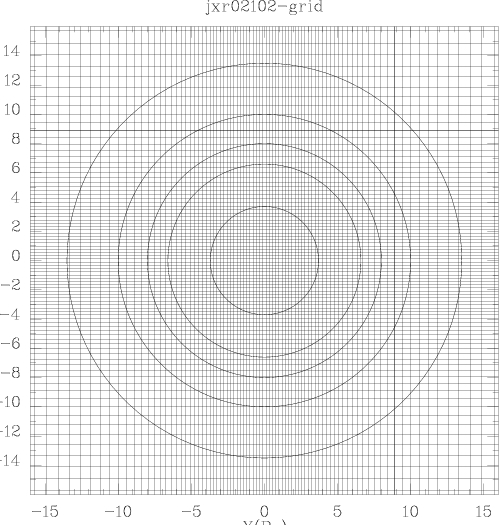
\includegraphics[scale=0.15]{images/StretchedCartesian.jpg}
\begin{itemize}
   \item[] \textbf{OpenGGCM}
   \item Stretched cartesian grid.
   \item Solves resistive MHD. (Not neglecting magnetic diffusivity)
   \item Conservative finite difference.
\end{itemize} &

\centering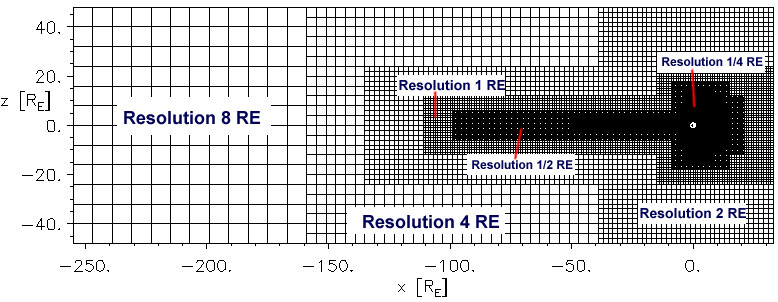
\includegraphics[scale=0.15]{images/BATS-R-US_Grid.jpg}
\begin{itemize}
  \item[] \textbf{BATS-R-US/SWMF}
  \item Block adaptive grid.
  \item Solves ideal MHD.
  \item Finite volumes.
  \item SWMF adds Rice Convection Model.
\end{itemize}
\end{tabular}
\end{frame}
\section{Validation}

\subsection{Overview}
\begin{frame}
	\begin{itemize}
	  \item \textbf{Verification} analyses ensure that the numerical implementation
	  of the mathematics are correct.
	  \begin{itemize}
	    \item Verification done extensively by model developers.
	  \end{itemize}
	  \item \textbf{Validation} analysis encompasses many ways of looking at model
	  outputs.
	  \begin{itemize}
	    \item 15 methods used (\textit{Sargent}, 2003).
	  \end{itemize}
	\end{itemize}
\end{frame}

\subsection{Validation Methods}
\begin{frame}
\frametitle{Validation}
\begin{tabular}{p{0.4\textwidth}p{0.5\textwidth}}
\begin{itemize}
  \item Animation
  \item \textbf{Comparison to other models}
  \item Degenerative tests
  \item Event validity
  \item Extreme condition test
  \item Face validity
  \item Historical data validation
  \item Historical methods
\end{itemize}&
\begin{itemize}
  \item Internal validity
  \item Multistage validation
  \item Operational graphics
  \item \textbf{Parameter variability - sensitivity analysis}
  \item Predictive validation
  \item Traces
  \item Turing tests
\end{itemize}
\end{tabular}
\end{frame}

\begin{frame}
	\begin{itemize}
	  \item \textbf{Comparison to other models}: The results from other already
  validated models are used to determine a new models' validity.
	  \item \textbf{Parameter variability - sensitivity analysis}: Changing the
  input and internal values of a model to determine the effect of the models
  output/behavior.
	\end{itemize}
\end{frame}
\section{Experiments}

\againframe{Motivation}
% Difficult to model the magnetosphere over an 11 year cycle today, GEM
% challenge is only 6-8 events, each event is unique, documenting the tendencies
% of models gives a reference to model developers as to why a model does poorly

\againframe{Experiments}

\subsection{$B_z$ Reversal}
\begin{frame}
	\frametitle{Experiment Setup}
	\begin{itemize}
 	 \item $B_z$ reversal from positive to negative at 00:30 out of 06:00. 
 	 \item Other input variables kept at 11 year means.
 	\begin{table}
 	\small
	\begin{center}
  	\caption{Chosen values for CCMC run 1}
  	\begin{tabular}{| l | c | c | c | c | }
    \hline
    \textbf{Run Num.} & \textbf{$\rho$} [$cm^{-3}$] & \textbf{$T$} [$K$] &
    \textbf{$U_x$} [$km/s$] &
    \textbf{$B_z$} [$nT$]
    \\
    \hline 
    1 & 5.76 & 101289 & -442  & +3.1 to -3.0 at 00:30 \\ \hline
  \end{tabular}
  \label{table:runs12}
\end{center}
\end{table}
	\begin{figure}
		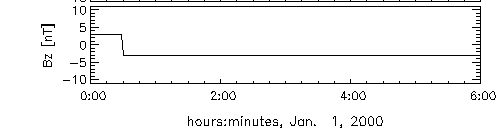
\includegraphics[scale=0.3]{images/CCMCRun1.png}
		\caption{CCMC run 1 plot of input time series }
	\end{figure}
	\end{itemize}
\end{frame}

\begin{frame}
	\frametitle{Input Variable Selection}\
	\begin{figure}
		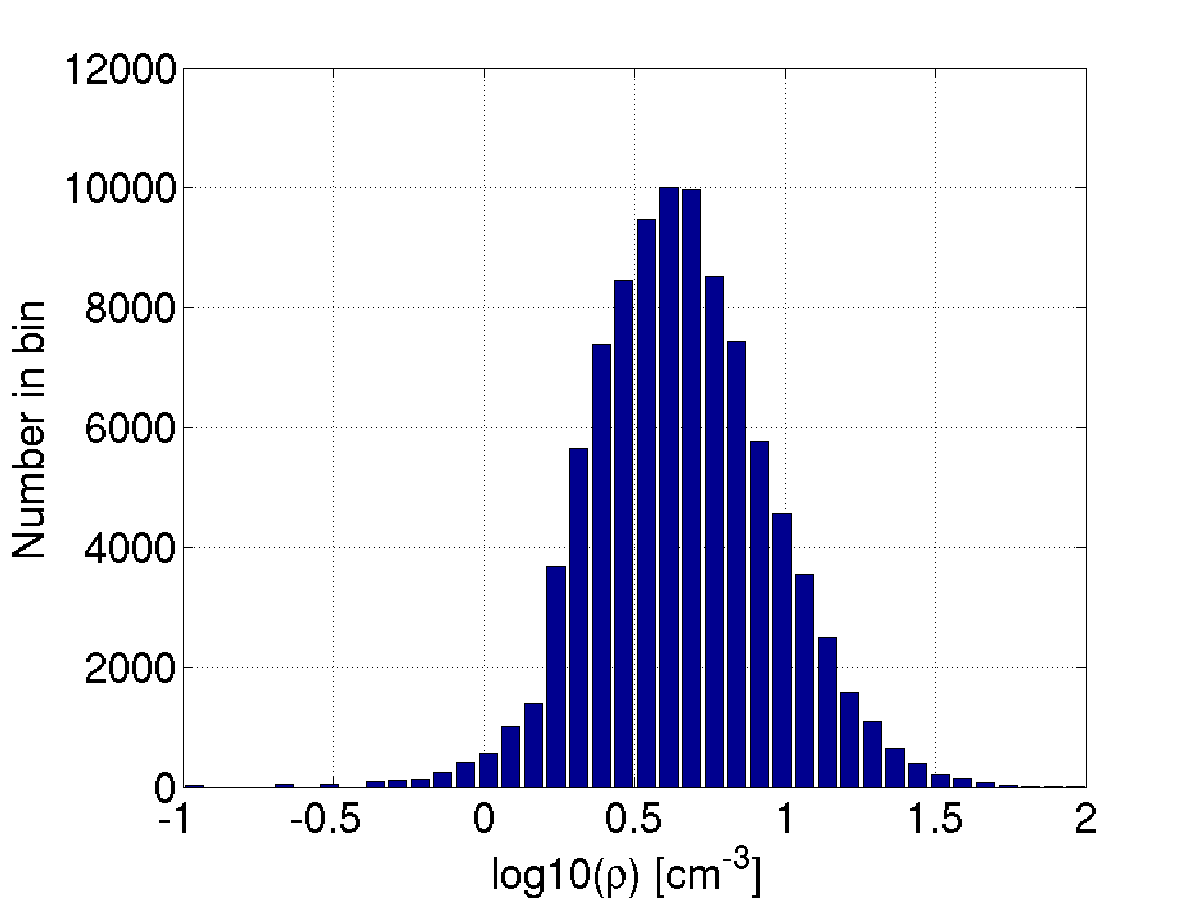
\includegraphics[scale=0.17]{images/hist_N.png}\quad
		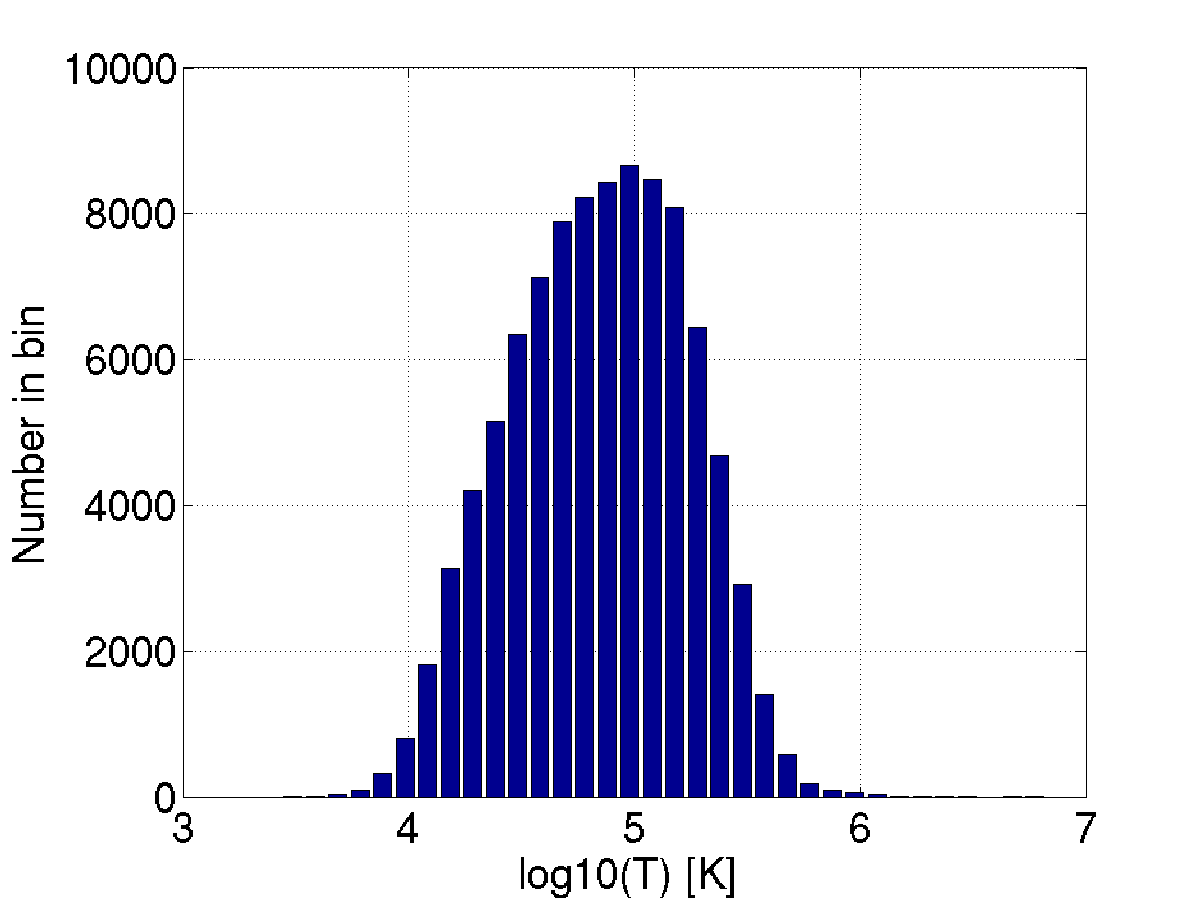
\includegraphics[scale=0.17]{images/hist_T.png}\\
		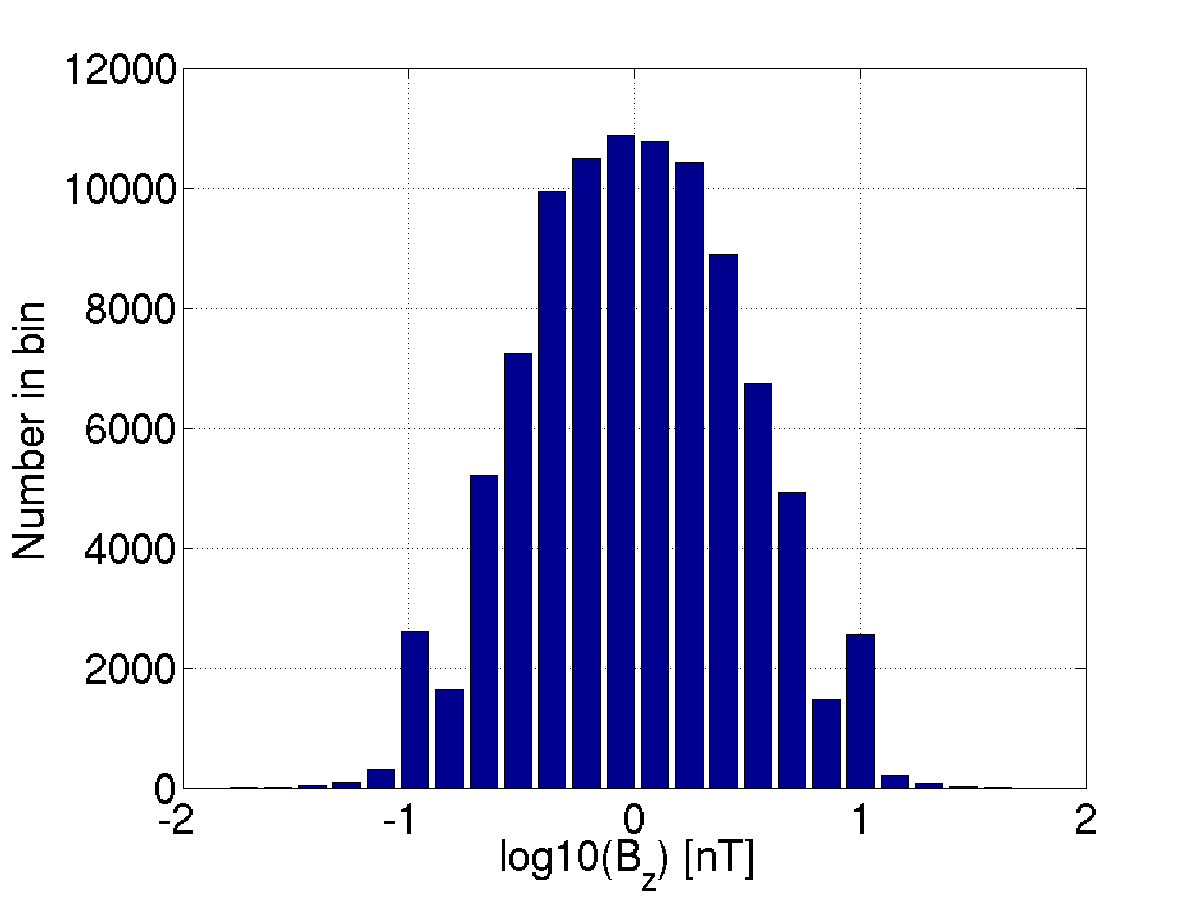
\includegraphics[scale=0.17]{images/hist_BZ.png}\quad
		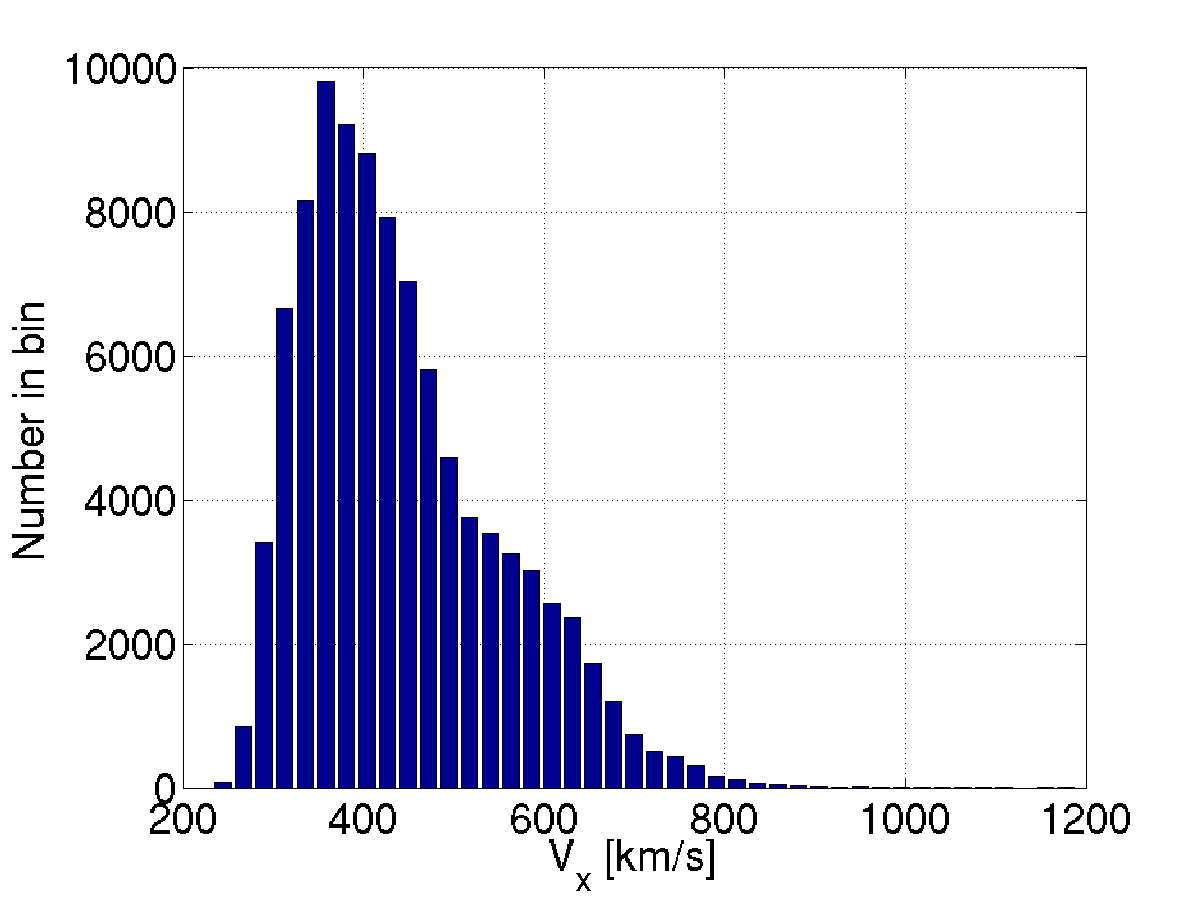
\includegraphics[scale=0.17]{images/hist_V.png}\\
		\caption{Jan 1, 2000 to Jan 1, 2011 Histograms of ACE Data }
\end{figure}
\end{frame}

\begin{frame}
\frametitle{$B_z$ Analysis: Magnetopause locations}
\begin{itemize}
  \item Important for satellite operations. Avoid crossing from magnetosphere
  into solar wind.
  \item For this experiment:
  \begin{itemize}
    \item No ring current and northward IMF $B_z$
    \item No ring current and southward IMF $B_z$
    \item Included ring current and northward IMF $B_z$
    \item Included ring current and southward IMF $B_z$
  \end{itemize}
\end{itemize}
\end{frame}

\begin{frame}
	\frametitle{No ring current and northward IMF $B_z$}
	\begin{columns}
	\begin{column}{.6\textwidth}
	\begin{figure}
		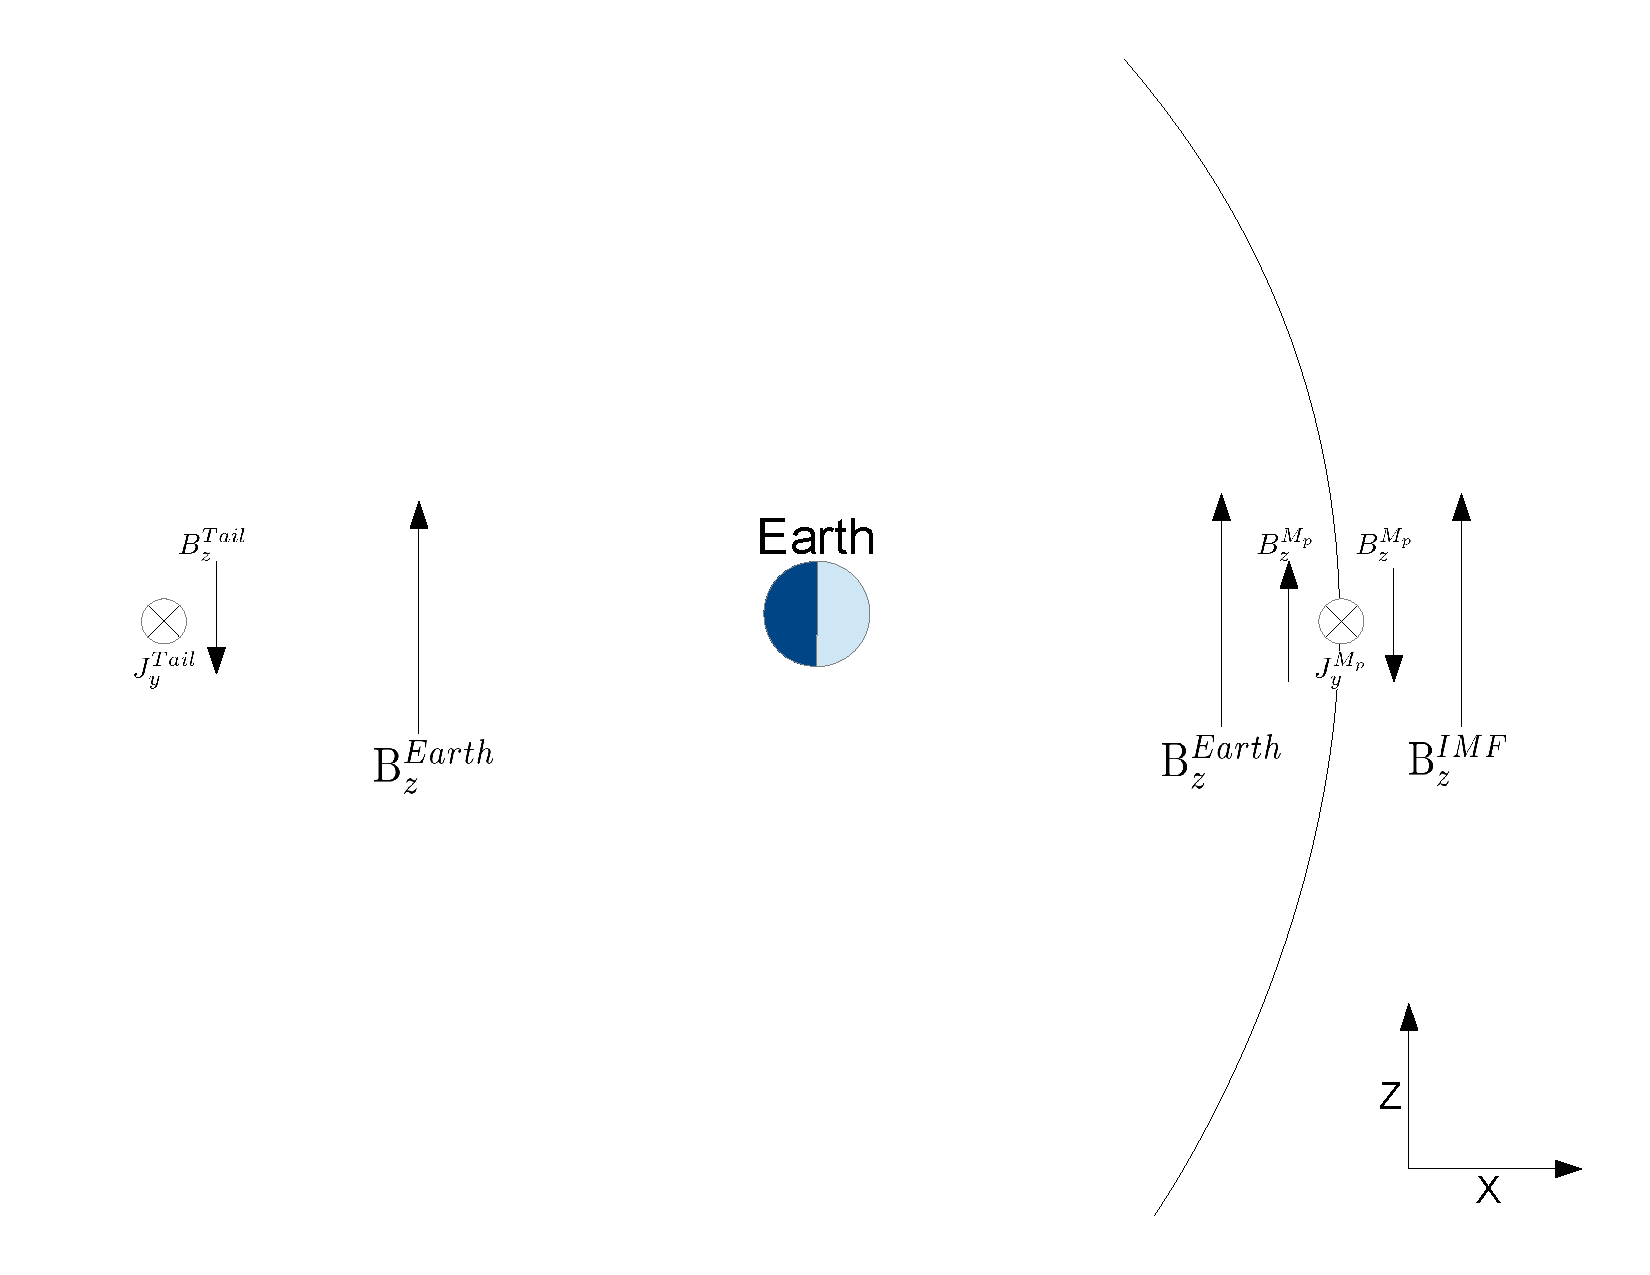
\includegraphics[scale=.23]{images/NimfNoRC.pdf}
	\end{figure}
	\end{column}
	\begin{column}{.4\textwidth}
	\begin{figure}
		\textbf{BATS-R-US $B_z$}\\
		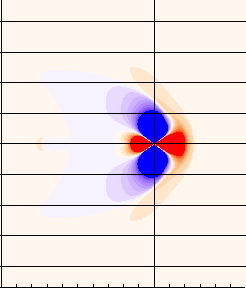
\includegraphics[scale=.45]{images/NBzNoRCM.png}
	\end{figure}
	\end{column}
	\end{columns}
\end{frame}

\begin{frame}
	\frametitle{No ring current and southward IMF $B_z$}
	\begin{columns}
	\begin{column}{.6\textwidth}
	\begin{figure}
		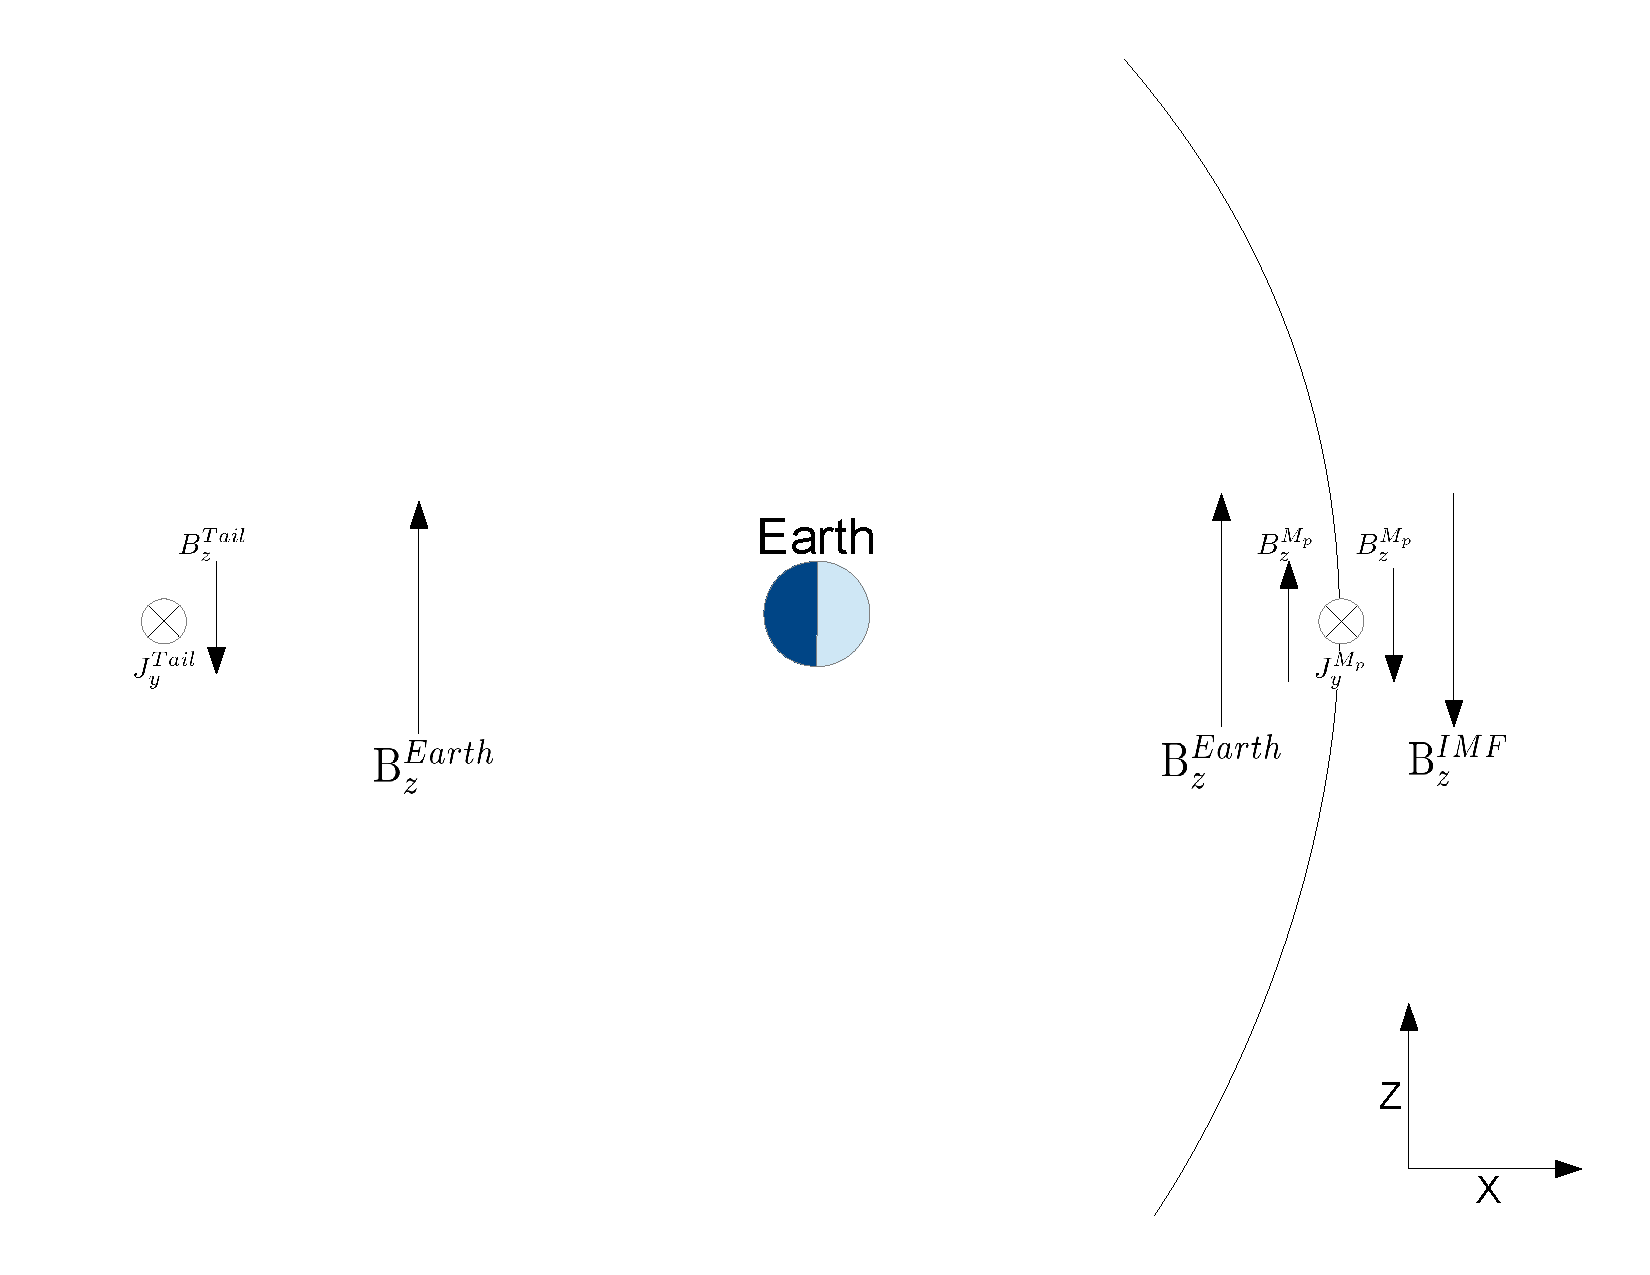
\includegraphics[scale=.23]{images/SimfNoRC.pdf}
	\end{figure}
	\end{column}
	\begin{column}{.4\textwidth}
	\begin{figure}
	\textbf{BATS-R-US $B_z$}\\
	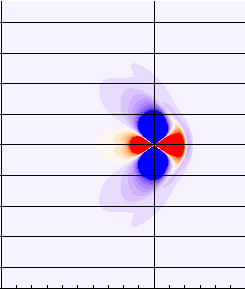
\includegraphics[scale=.45]{images/SBzNoRCM.png}
	\end{figure}
	\end{column}
	\end{columns}
\end{frame}

\begin{frame}
	\frametitle{Included ring current and northward IMF $B_z$}
	\begin{columns}
	\begin{column}{.6\textwidth}
	\begin{figure}
		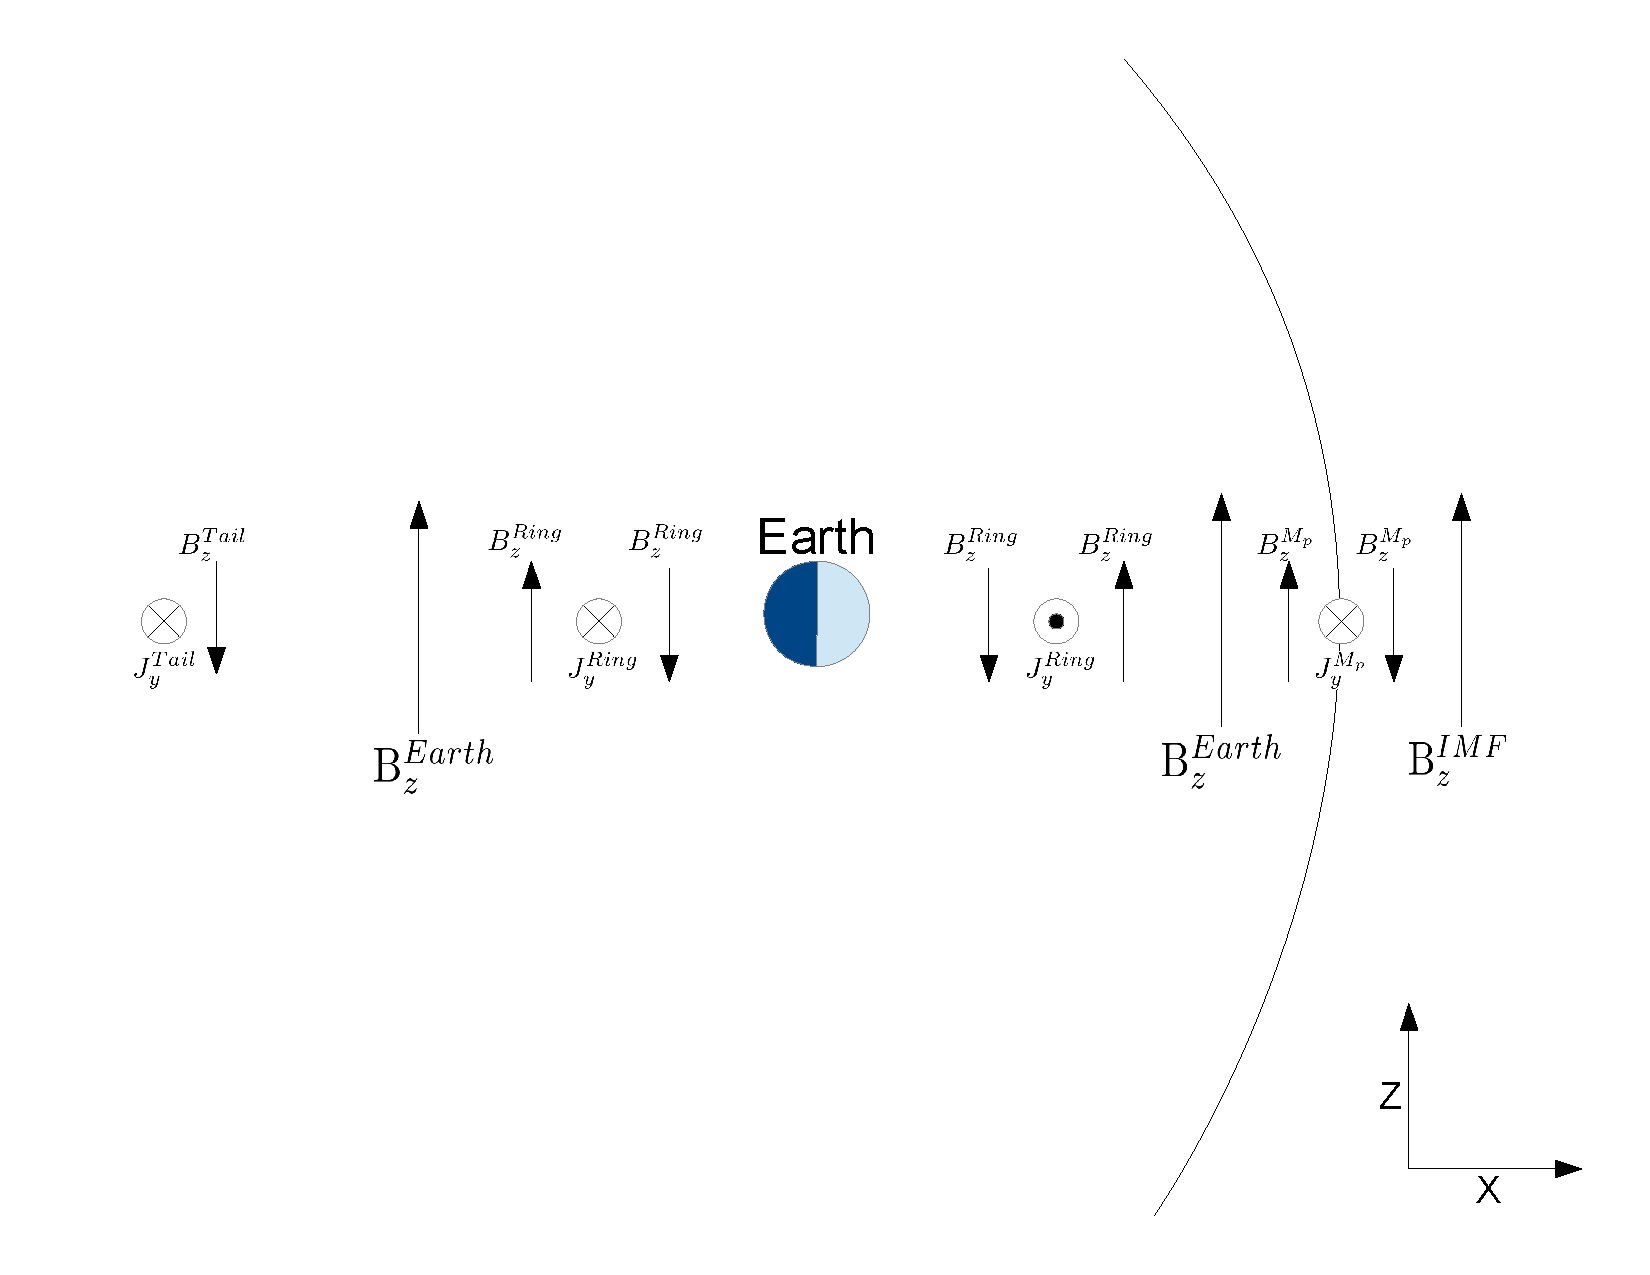
\includegraphics[scale=.23]{images/NimfRC.pdf}
		
	\end{figure}
	\end{column}
	\begin{column}{.4\textwidth}
	\begin{figure}
		\textbf{SWMF $B_z$}\\
		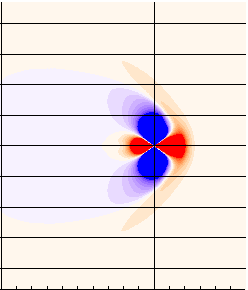
\includegraphics[scale=.45]{images/NBzRCM.png}
	\end{figure}
	\end{column}
	\end{columns}
\end{frame}

\begin{frame}
	\frametitle{Included ring current and southward IMF $B_z$}
	\begin{columns}
	\begin{column}{.6\textwidth}
	\begin{figure}
		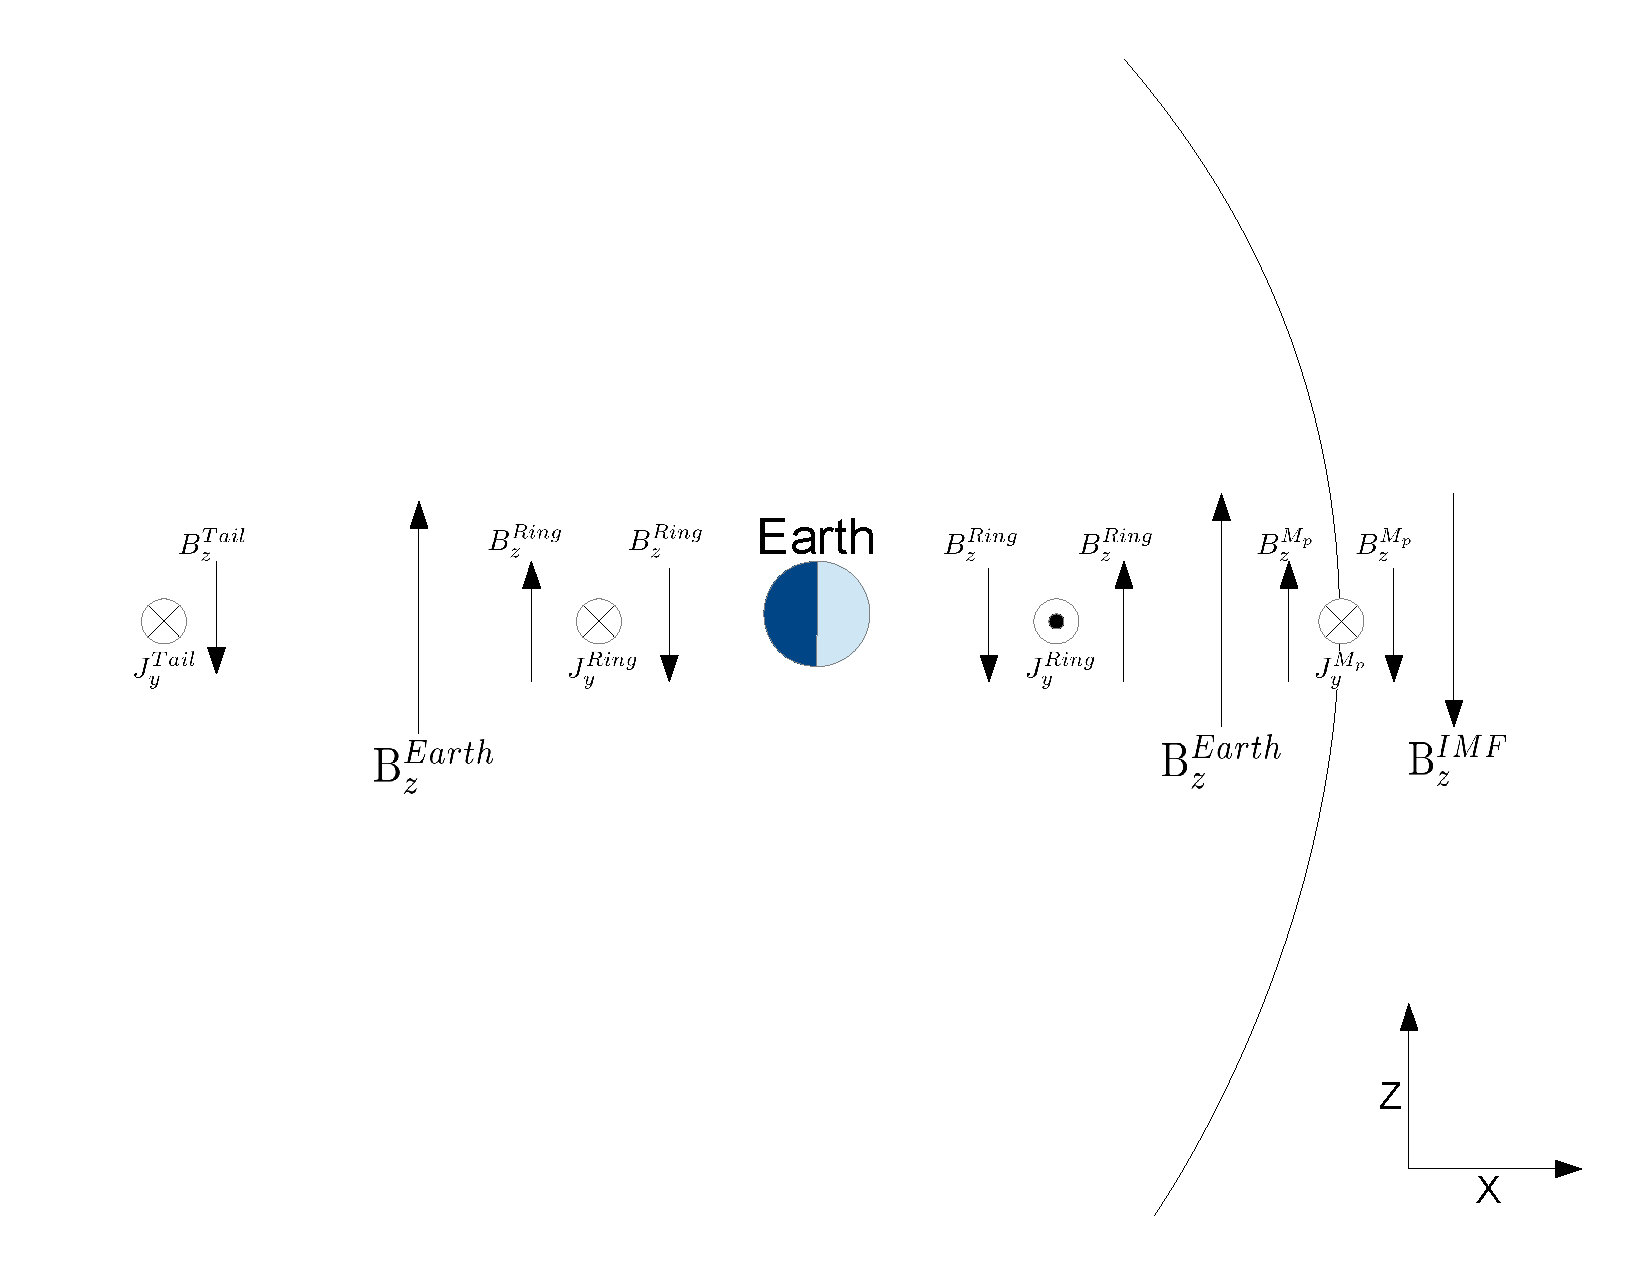
\includegraphics[scale=.23]{images/SimfRC.pdf}
	\end{figure}
	\end{column}
	\begin{column}{.4\textwidth}
	\begin{figure}
		\textbf{SWMF $B_z$}\\
		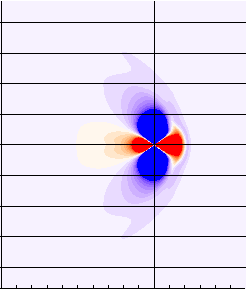
\includegraphics[scale=.45]{images/SBzRCM.png}
	\end{figure}
	\end{column}
	\end{columns}
\end{frame}

\begin{frame}
\frametitle{$B_z$ Differences}
\begin{center}
\begin{figure}
\includegraphics[scale=0.15]{/mnt/Disk2/Brian_Curtis_042213_1/Results/images/Bz_File5.png}\\
\includegraphics[scale=0.15]{/mnt/Disk2/Brian_Curtis_042213_2/Results/images/Bz_File5.png}\\
\caption{OpenGGCM (top) and BATS-R-US (bottom) northward IMF $B_z$}
\end{figure}
\end{center}
\end{frame}


\begin{frame}
\frametitle{$B_z$ Differences}
\begin{center}
\begin{figure}
\href{images/1_ReversalB.pdf}{\includegraphics[scale=0.3]{/mnt/Disk2/Results/0_1/images/Bz_Diff_File5.png}}\\
\caption{OpenGGCM - BATS-R-US $B_z$ Percent Diff }
\end{figure}
\end{center}
\end{frame}

\begin{frame}
\frametitle{$B_z$ Differences}
\begin{center}
\begin{figure}
\includegraphics[scale=0.15]{/mnt/Disk2/Results/0_2/images/Bz_Diff_File5.png}\\
\includegraphics[scale=0.15]{/mnt/Disk2/Results/1_2/images/Bz_Diff_File5.png}\\
\caption{OpenGGCM - SWMF (top) and BATS-R-US - SWMF (bottom) northward IMF
$B_z$ differences}
\end{figure}
\end{center}
\end{frame}

\begin{frame}
\frametitle{$B_z$ Differences}
\begin{center}
\begin{figure}
\includegraphics[scale=0.15]{/mnt/Disk2/Results/0_2/images/Bz_Diff_File30.png}\\
\includegraphics[scale=0.15]{/mnt/Disk2/Results/1_2/images/Bz_Diff_File30.png}\\
\caption{OpenGGCM - SWMF (top) and BATS-R-US - SWMF (bottom) southward IMF
$B_z$ differences}
\end{figure}
\end{center}
\end{frame}

\begin{frame}
\frametitle{$\rho$ Differences}
\begin{center}
\begin{figure}
\includegraphics[scale=0.15]{/mnt/Disk2/Brian_Curtis_042213_1/Results/images/rho_File5.png}\\
\includegraphics[scale=0.15]{/mnt/Disk2/Brian_Curtis_042213_3/Results/images/rho_File5.png}\\
\caption{OpenGGCM (top) and SWMF (bottom) $\rho$}
\end{figure}
\end{center}
\end{frame}


\begin{frame}
\frametitle{$\rho$ Differences}
\begin{center}
\begin{figure}
\includegraphics[scale=0.3]{/mnt/Disk2/Results/0_2/images/rho_Diff_File5.png}\\
\caption{OpenGGCM - SWMF $\rho$ Percent Diff}
\end{figure}
\end{center}
\end{frame}

\begin{frame}
\frametitle{Expected $U_x$}
\begin{figure}
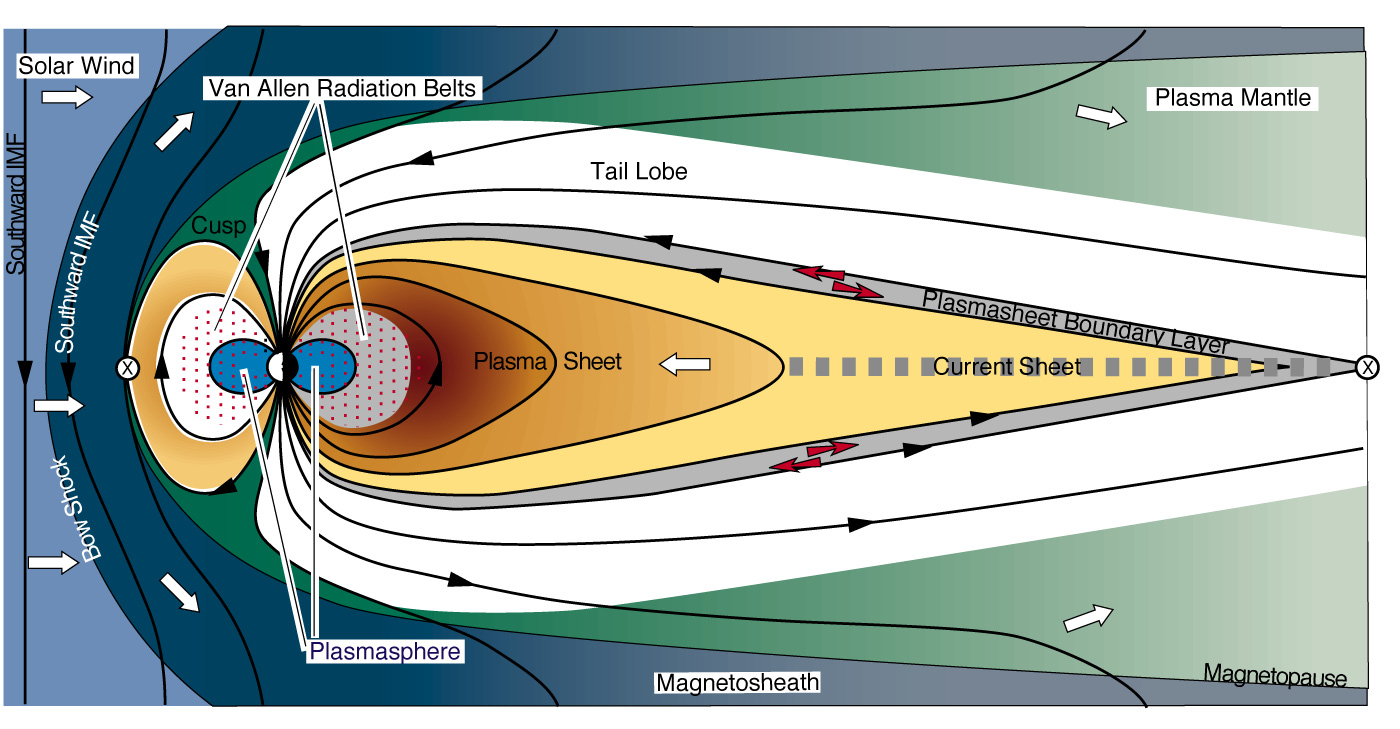
\includegraphics[scale=0.21]{images/Rice_Magnetosphere.jpg}\\
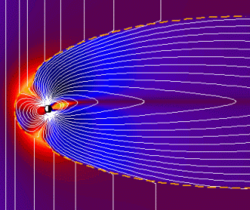
\includegraphics[scale=0.4]{images/tsyganenko.png}
\end{figure}
\end{frame}

\begin{frame}
\frametitle{$U_x$ Plots}
\begin{center}
\begin{figure}
\includegraphics[scale=0.15]{/mnt/Disk2/Brian_Curtis_042213_2/Results/images/Ux_File5.png}\\
\includegraphics[scale=0.15]{/mnt/Disk2/Brian_Curtis_042213_3/Results/images/Ux_File5.png}\\
\caption{BATS-R-US (top) and SWMF (bottom) $U_x$}
\end{figure}

\end{center}
\end{frame}


\begin{frame}
\frametitle{$U_x$ Differences}
\begin{center}
\begin{figure}
\includegraphics[scale=0.3]{/mnt/Disk2/Results/1_2/images/Ux_Diff_File5.png}\\
\caption{BATS-R-US - SWMF $U_x$ Percent Diff}
\end{figure}
\end{center}
\end{frame}

\begin{frame}[shrink]
\frametitle{$B_z$ Reversal Conclusions}
For a reversal in IMF $B_z$, the following occur in the models:
\begin{itemize}
  \item The OpenGGCM magnetopause is closest to Earth as it has the weakest
  magnetic pressure near-Earth.
  \item In positive IMF $B_z$ conditions, the ring current pushes the SWMF
  magnetopause farther Sunward than the BATS-R-US.
  \item In negative IMF $B_z$ conditions, the SWMF magnetopause is farther
  Earthward than the BATS-R-US.
  \item The differences in magnetopause positions between the BATS-R-US and SWMF
  are due to the effects of the ring current addition to the magnetosphere in
  the SWMF model.
  \item Densities are highest with the SWMF and lowest with the OpenGGCM.
  \item The OpenGGCM tail velocities are largely different from the BATS-R-US
  and SWMF.
\end{itemize}
\end{frame}

\subsection{Preconditioning}

\begin{frame}
\frametitle{Preconditioning Definition}
\textbf{Definition:} Magnetospheric model pre-conditioning takes an
initial state, then the model is iterated through time and conditions are slowly
changed to meet the initial conditions set by the user.
\begin{itemize}
  \item Earth's magnetic field is set as a dipole, mirror dipole at ~16$R_e$. Plasma temperature and density initially set to 5000 [$K$] and 0.1
  [$cm^{-3}$] respectively.
  \item OpenGGCM: Uses 2 hours of preconditioning that includes 30 minutes with
  negative Bz.
  \item BATS-R-US/SWMF: Uses a local time stepping scheme where an approximate
  steady state is reached after 2500 iteration steps.
\end{itemize}
\end{frame}

\begin{frame}[shrink]
\frametitle{Experiment Setup}
\begin{itemize}
  \item First run: $B_z$ reversal at 00:30 (early reversal)
  \item Second run: Delay $B_z$ reversal until 02:00 (late reversal)
  \item Take equal data sample sizes matching the reversal times.
  \item Compare models with themselves at two different reversal times.
\end{itemize}
\end{frame}

\begin{frame}
\frametitle{Model Outputs}
\begin{tabular}{p{0.4\textwidth}p{0.5\textwidth}}
\begin{itemize}
  \item[]
  \includegraphics[scale=0.10]{/mnt/Disk2/Precondition/Results/0_3/images/Ux_Diff_File5.png}
  \item[]
  \includegraphics[scale=0.10]{/mnt/Disk2/Precondition/Results/1_4/images/Ux_Diff_File5.png}
  \item[]
  \includegraphics[scale=0.10]{/mnt/Disk2/Precondition/Results/2_5/images/Ux_Diff_File5.png}
\end{itemize}
 &
\begin{itemize}
  \setlength{\itemsep}{43pt}
  \item \href{images/2_PreconditionOpenGGCM.pdf}{OpenGGCM}
  \item \href{images/3_PreconditionBATSRUS.pdf}{BATS-R-US}
  \item \href{images/4_PreconditionSWMF.pdf}{SWMF}
\end{itemize}
\end{tabular}
\end{frame}

\begin{frame}[shrink]
\frametitle{Preconditioning Conclusions}
For changes in the preconditioning time of magnetospheric MHD models the
following shows that there is a significant sensitivity to preconditioning time
and supports that there is a need for a more detailed analysis:
\begin{itemize}
  \item Longer preconditioning time allowed the magnetosphere to relax more
  giving different positions for the magnetopause with all three models.
  \item The OpenGGCM magnetopause position differences were wider than that of
  SWMF or BATS-R-US.
  \item There were large differences for all three models before the $B_z$
  reversal.
  \item The differences in the current sheet region for the OpenGGCM were
  similar before and after the reversal.
  \item The BATS-R-US and SWMF differences decreased after the $B_z$ reversal to
  near zero.
\end{itemize}
\end{frame}

\subsection{Extreme Conditions}

\begin{frame}
\frametitle{Experiment Setup}
\begin{table}
\begin{center}
  \caption{Chosen values for CCMC runs 3 and 4}
  \begin{tabular}{| l | c | c | c | c | }
    \hline
    \textbf{Run Num.} & \textbf{$\rho$} & \textbf{$T$} & \textbf{$Vx$} &
    \textbf{$B_z$}
    \\
    \hline 
    3 & 11 & 101289 & -604  & -3.0 \\ \hline
    4 & 2 & 101289 & -320  & 3.1 \\ \hline
  \end{tabular}
  \label{table:runs34}
\end{center}
\end{table}
\begin{tabular}{p{0.5\textwidth}p{0.5\textwidth}}
\begin{itemize}
  \item[]\includegraphics[scale=0.12]{/mnt/Disk2/Brian_Curtis_042413_1/Results/images/Bz_File5.png}\\
  \item[] Run 3 - High Compression
\end{itemize}
 &
\begin{itemize}
  \item[]\includegraphics[scale=0.12]{/mnt/Disk2/Brian_Curtis_042413_5/Results/images/Bz_File5.png}\\
  \item[] Run 4 - Low Compression
\end{itemize}
\end{tabular}
\end{frame}

\begin{frame}
\frametitle{Low Compression - Model Output}
\begin{columns}
\begin{column}{.33\textwidth}
\begin{figure}
	\textbf{$B_z$ Percent Diff}\\
	\includegraphics[scale=0.10]{/mnt/Disk2/Results/0_1/images/Bz_Diff_File5.png}\\
  	\includegraphics[scale=0.10]{/mnt/Disk2/Results/0_2/images/Bz_Diff_File5.png}\\
  	\includegraphics[scale=0.10]{/mnt/Disk2/Results/1_2/images/Bz_Diff_File5.png}
\end{figure}
\end{column}
&
\begin{column}{.33\textwidth}
\begin{figure}
	\textbf{$\rho$ Percent Diff}\\
	\includegraphics[scale=0.10]{/mnt/Disk2/Results/0_1/images/rho_Diff_File5.png}\\
  	\includegraphics[scale=0.10]{/mnt/Disk2/Results/0_2/images/rho_Diff_File5.png}\\
  	\includegraphics[scale=0.10]{/mnt/Disk2/Results/1_2/images/rho_Diff_File5.png}
\end{figure}
\end{column}
&
\begin{column}{.33\textwidth}
\begin{figure}
	\textbf{$U_x$ Percent Diff}\\
	\includegraphics[scale=0.10]{/mnt/Disk2/Results/0_1/images/Ux_Diff_File5.png}\\
  	\includegraphics[scale=0.10]{/mnt/Disk2/Results/0_2/images/Ux_Diff_File5.png}\\
  	\includegraphics[scale=0.10]{/mnt/Disk2/Results/1_2/images/Ux_Diff_File5.png}
\end{figure}
\end{column}
\end{columns}
\end{frame}

\begin{frame}
\frametitle{High Compression - Model Output}
\begin{tabular}{p{0.4\textwidth}p{0.5\textwidth}}
\begin{itemize}
  \item[]
  \includegraphics[scale=0.10]{/mnt/Disk2/Brian_Curtis_042413_1/Results/images/Ux_File5.png}
  \item[]
  \includegraphics[scale=0.10]{/mnt/Disk2/Brian_Curtis_042413_2/Results/images/Ux_File5.png}
  \item[]
  \includegraphics[scale=0.10]{/mnt/Disk2/Brian_Curtis_042413_3/Results/images/Ux_File5.png}
\end{itemize}
 &
\begin{itemize}
  \setlength{\itemsep}{43pt}
  \item \href{images/5_HighOpenGGCM.pdf}{OpenGGCM}
  \item \href{images/6_HighBATSRUS.pdf}{BATS-R-US}
  \item \href{images/7_HighSWMF.pdf}{SWMF}
\end{itemize}
\end{tabular}
\end{frame}

\begin{frame}[shrink]
\frametitle{Extreme Conditions Conclusions}
For extreme conditions in the solar wind, the
following occurs in the magnetosphere:
\begin{itemize}
  \item The OpenGGCM has a large region of Earthward $U_x$ in the current sheet
  region that grows as time progresses in a compressed environment.
  \item The BATS-R-US is either completely stable or stops in a compressed
  environment.
  \item In a compressed environment the SWMF will eventually oscillate.
  \item The OpenGGCM has the highest tailward velocities in a compressed
  environment.
  \item The ring current reduced the maximum velocities in the SWMF.
  \item The OpenGGCM has the highest $B_z$ in a compressed environment.
  \item All three models have similar magnetopause positions in a low
  compression environment.
  \item The OpenGGCM current sheet velocities are largest in a low compression
  environment.
\end{itemize}
\end{frame}

\section{Summary}

\againframe{Motivation}

\againframe{Summary}

\subsection{Future Work}

\begin{frame}
\frametitle{Future Work}
\begin{itemize}
  \item Expand to more magnetospheric models.
  \item Increased preconditioning time can allow more stability in the
  magnetosphere. Research is needed to better understand a more appropriate
  preconditioning time.
  \item Expand to different types of conditions.
  \item Correlate model differences to real-time outputs for forecasters.
\end{itemize}
\end{frame}

\begin{frame}
\frametitle{Thank you.}
\end{frame}


\begin{frame}
\frametitle{Appendix - MHD}

\begin{itemize}
  \item Conservation of Mass.\\
    $\frac{\partial\rho}{\partial t} + \nabla \cdot (\rho \mathbf{u}) = 0$
  \item Conservation of Momentum.\\
    $\frac{\partial \rho \mathbf{u}}{\partial t} + \nabla \cdot (\rho
\mathbf{u u}) + \nabla \cdot P - \rho_q\mathbf{E} - \mathbf{J}
\times \mathbf{B} - \rho \mathbf{g} = 0$
  \item Conservation of Energy.\\
    $\frac{\partial \epsilon}{\partial t} + \nabla \cdot (\epsilon \mathbf{u} + P
\cdot \mathbf{u} + \mathbf{q}) - \mathbf{J} \cdot \mathbf{E} - \rho\mathbf{u}
\cdot \mathbf{g} = 0$
  \item Maxwell's Equations:
  \begin{itemize}
    \item Gauss' Law.\\
    $ \nabla \cdot \mathbf{E} = \frac{\rho_q}{\epsilon_0}$
    \item Gauss' Law for Magnetism.\\
    $ \nabla \cdot \mathbf{B} = 0 $
    \item Faraday's Law.\\
    $ \nabla \times \mathbf{E} = - \frac{\partial
\mathbf{B}}{\partial t} $
    \item Ampere's Law.\\
    $ \nabla \times \mathbf{B} = \mu_0(\mathbf{J} + \epsilon_0
\frac{\partial \mathbf{E}}{\partial t}) $
  \end{itemize}
\end{itemize}

\end{frame}

\begin{frame}
\frametitle{Appendix: Ideal MHD}
To simplify the single fluid MHD equations, the following assumptions were made:
\begin{itemize}
  \item The time derivative of E is small\\
  $\nabla \times \mathbf{B} = \mu_0 \mathbf{J}$
  \item Isotropic Pressure\\
  $\nabla \cdot P = \nabla p$ 
  \item Charge neutrality\\
  If net charge balances, then $\rho_q = 0$
  \item Neglect small terms\\
  If $p_e$ is small, then any term involving $P_q$ can be neglected
  \item Single ion flow with collision term approximation
  $\mathbf{J} = \sigma(\mathbf{E} + \mathbf{u} \times \mathbf{B})$
  \item Perfect conductivity\\
  $\frac{\partial \mathbf{B}}{\partial t} + \nabla \cdot (\mathbf{u}\mathbf{B}
  - \mathbf{B}\mathbf{u}) = 0$
\end{itemize}

\end{frame}

\end{document}
